\documentclass[spanish,letterpaper,oneside]{article}

\def\documenttitle {Universo 3-60}
\def\documentsubtitle {Temas selectos de matemáticas I · Cohorte SD26}
\def\documentsubject {Actividad 3 (Sesión 10) · Polígonos Inscritos, Ángulos Centrales e Inscritos}
\def\documentauthor {Mtro. Martín Jonathan de la Cruz Muñoz}
\def\coursename {Temas selectos de matemáticas I}
\def\coursecode {PFM02}

\def\universityname {Instituto de Investigación, Innovación y Estudios de Posgrado para la Educación del Estado de Nuevo León}
\def\universityfaculty {Maestría en Aprendizaje y Enseñanza de las Matemáticas}
\def\universitydepartment {Temas selectos de matemáticas I}
\def\universitydepartmentimage {img/iiiepe/marca-iiiepe.png}
\def\universitydepartmentimagecfg {height=1.75cm}
\def\universitylocation {Monterrey, Nuevo León}
\def\studentfullname {Mtro. Martín Jonathan de la Cruz Muñoz}
\def\studentid {00874}
\def\studentemail {martin.delacruz@campus.iiiepe.edu.mx}
\def\programperiod {2do periodo, agosto--noviembre de 2026 (SD26)}
\def\programmodality {Modalidad presencial y en línea}
\def\programshort {MAEM}

\def\authortable {
  \begin{tabular}{ll}
    \textbf{Alumno:} & \studentfullname \\
    Matrícula: & \studentid \\
    Correo institucional: & \studentemail \\
    Unidad: & \coursename \\
    Programa: & \programshort \\
    Periodo: & \programperiod \\
    & \\
    \multicolumn{2}{l}{Fecha de realización: 24 de octubre de 2026} \\
    \multicolumn{2}{l}{\universitylocation}
  \end{tabular}
}

\input{template}

\usepackage{helvet}
\renewcommand{\familydefault}{\sfdefault}
\usepackage{amsmath,amssymb,booktabs,array,longtable,pdflscape,tikz,tabularx,colortbl,pgfplots,enumitem,needspace}
\usepackage[most]{tcolorbox}
\usetikzlibrary{arrows.meta,positioning,calc,fit,backgrounds}
\pgfplotsset{compat=1.18}

\definecolor{iiiepeNavy}{HTML}{163B5C}
\definecolor{iiiepeBlue}{HTML}{1F6F9F}
\definecolor{iiiepeAqua}{HTML}{20B7A8}
\definecolor{iiiepeOrange}{HTML}{F28C28}
\definecolor{iiiepePaper}{HTML}{F6F8F7}
\definecolor{iiiepeInk}{HTML}{1E2A32}
\definecolor{iiiepePale}{HTML}{EEF5F8}
\def\portraittitlecolor {iiiepeNavy}
\setcitestyle{authoryear,open={(},close={)}}

\newcommand{\insertcoverwatermark}{%
  \AddToShipoutPictureBG*{%
    \begin{tikzpicture}[remember picture,overlay]
      \node[opacity=.06,inner sep=0pt] at (current page.center)
      {
\includegraphics[width=.58\paperwidth]{img/iiiepe/logo-puntos.png}};
    \end{tikzpicture}%
  }%
}

\newtcolorbox{propuestabox}[1][]{%
  enhanced,breakable,
  colback=iiiepePaper,colframe=iiiepeAqua!80!iiiepeNavy,
  boxrule=1pt,leftrule=4pt,arc=2pt,
  left=8pt,right=8pt,top=6pt,bottom=6pt,
  before skip=6pt,after skip=10pt,
  fonttitle=\bfseries\color{white},coltitle=white,
  colbacktitle=iiiepeNavy,
  attach boxed title to top left={xshift=8pt,yshift=-2pt},
  boxed title style={colback=iiiepeNavy,colframe=iiiepeNavy,arc=1pt},
  title={Propuesta didáctica},#1}

\setlength{\parskip}{5pt}\setlength{\parindent}{0pt}
\begin{document}\insertcoverwatermark\templatePortrait\templatePagecfg\templateFinalcfg\fancyfoot{}\fancyfoot[L]{\scriptsize IIIEPE · MAEM · SD26}\fancyfoot[C]{\scriptsize\thepage}\fancyfoot[R]{\scriptsize Actividad 3}\setstretch{1.25}\raggedbottom

\section{Exploración presencial: triángulos y polígonos regulares}

\subsection{Suma de ángulos interiores de un triángulo (Diapositiva 10)}
Al recortar las tres esquinas (ángulos interiores $\alpha, \beta, \gamma$) de cualquier triángulo y reunir sus vértices sobre un punto común de apoyo, los tres sectores forman invariablemente un \textbf{ángulo llano} ($180^\circ$). Este hallazgo manipulativo coincide con el teorema euclidiano de paralelas: trazando por un vértice la paralela al lado opuesto, los ángulos alternos internos reproducen $\alpha$ y $\beta$ adyacentes a $\gamma$, verificando $\alpha + \beta + \gamma = 180^\circ$.

\subsection{Triangulación por diagonales desde un vértice (Diapositiva 14)}
Trazando las diagonales posibles desde un único vértice en un polígono convexo de $n$ lados se obtienen exactamente $n - 3$ diagonales que particionan el interior en $n - 2$ triángulos disjuntos. Como cada triángulo suma $180^\circ$, la suma de ángulos interiores es $S_{\text{int}}(n) = (n - 2)\cdot 180^\circ$.

{\small\setstretch{1.08}\renewcommand{\arraystretch}{1.18}
\begin{longtable}{|>{\raggedright\arraybackslash}p{0.25\linewidth}|>{\centering\arraybackslash}p{0.20\linewidth}|>{\centering\arraybackslash}p{0.23\linewidth}|>{\centering\arraybackslash}p{0.28\linewidth}|}\hline
\rowcolor{iiiepePale} \textbf{Polígono} & \textbf{Lados ($n$)} & \textbf{Triángulos ($n-2$)} & \textbf{Suma ángulos interiores} \\\hline
\endfirsthead\hline
\rowcolor{iiiepePale} \textbf{Polígono} & \textbf{Lados ($n$)} & \textbf{Triángulos ($n-2$)} & \textbf{Suma ángulos interiores} \\\hline
\endhead
Triángulo & $3$ & $1$ & $180^\circ$ \\\hline
Cuadrilátero & $4$ & $2$ & $360^\circ$ \\\hline
Pentágono & $5$ & $3$ & $540^\circ$ \\\hline
Hexágono & $6$ & $4$ & $720^\circ$ \\\hline
Heptágono & $7$ & $5$ & $900^\circ$ \\\hline
Octágono & $8$ & $6$ & $1080^\circ$ \\\hline
Eneágono & $9$ & $7$ & $1260^\circ$ \\\hline
Decágono & $10$ & $8$ & $1440^\circ$ \\\hline
\textbf{Icoságono (extensión)} & $\mathbf{20}$ & $\mathbf{18}$ & $\mathbf{3240^\circ}$ \\\hline
\end{longtable}}

\subsection{Polígonos regulares inscritos en circunferencias (Diapositiva 20)}
Al dividir el giro completo de $360^\circ$ entre $n$ vértices equiespaciados sobre una circunferencia, cada ángulo central mide $\theta_c = \frac{360^\circ}{n}$ y cada ángulo interior mide $\theta_i = \frac{(n-2)\cdot 180^\circ}{n} = 180^\circ - \frac{360^\circ}{n}$.

{\small\setstretch{1.08}\renewcommand{\arraystretch}{1.18}
\begin{longtable}{|>{\raggedright\arraybackslash}p{0.23\linewidth}|>{\centering\arraybackslash}p{0.14\linewidth}|>{\centering\arraybackslash}p{0.19\linewidth}|>{\centering\arraybackslash}p{0.23\linewidth}|>{\centering\arraybackslash}p{0.19\linewidth}|}\hline
\rowcolor{iiiepePale} \textbf{Polígono} & \textbf{Lados ($n$)} & \textbf{Ángulo central} & \textbf{Suma interiores} & \textbf{Cada interior} \\\hline
\endfirsthead\hline
\rowcolor{iiiepePale} \textbf{Polígono} & \textbf{Lados ($n$)} & \textbf{Ángulo central} & \textbf{Suma interiores} & \textbf{Cada interior} \\\hline
\endhead
Hexágono & $6$ & $60^\circ$ & $720^\circ$ & $120^\circ$ \\\hline
Octágono & $8$ & $45^\circ$ & $1080^\circ$ & $135^\circ$ \\\hline
Eneágono & $9$ & $40^\circ$ & $1260^\circ$ & $140^\circ$ \\\hline
Decágono & $10$ & $36^\circ$ & $1440^\circ$ & $144^\circ$ \\\hline
Dodecágono & $12$ & $30^\circ$ & $1800^\circ$ & $150^\circ$ \\\hline
Pentadecágono & $15$ & $24^\circ$ & $2340^\circ$ & $156^\circ$ \\\hline
Octadecágono & $18$ & $20^\circ$ & $2880^\circ$ & $160^\circ$ \\\hline
Icoságono & $20$ & $18^\circ$ & $3240^\circ$ & $162^\circ$ \\\hline
Icositetrágono & $24$ & $15^\circ$ & $3960^\circ$ & $165^\circ$ \\\hline
\end{longtable}}

\begin{figure}[htbp]
\centering
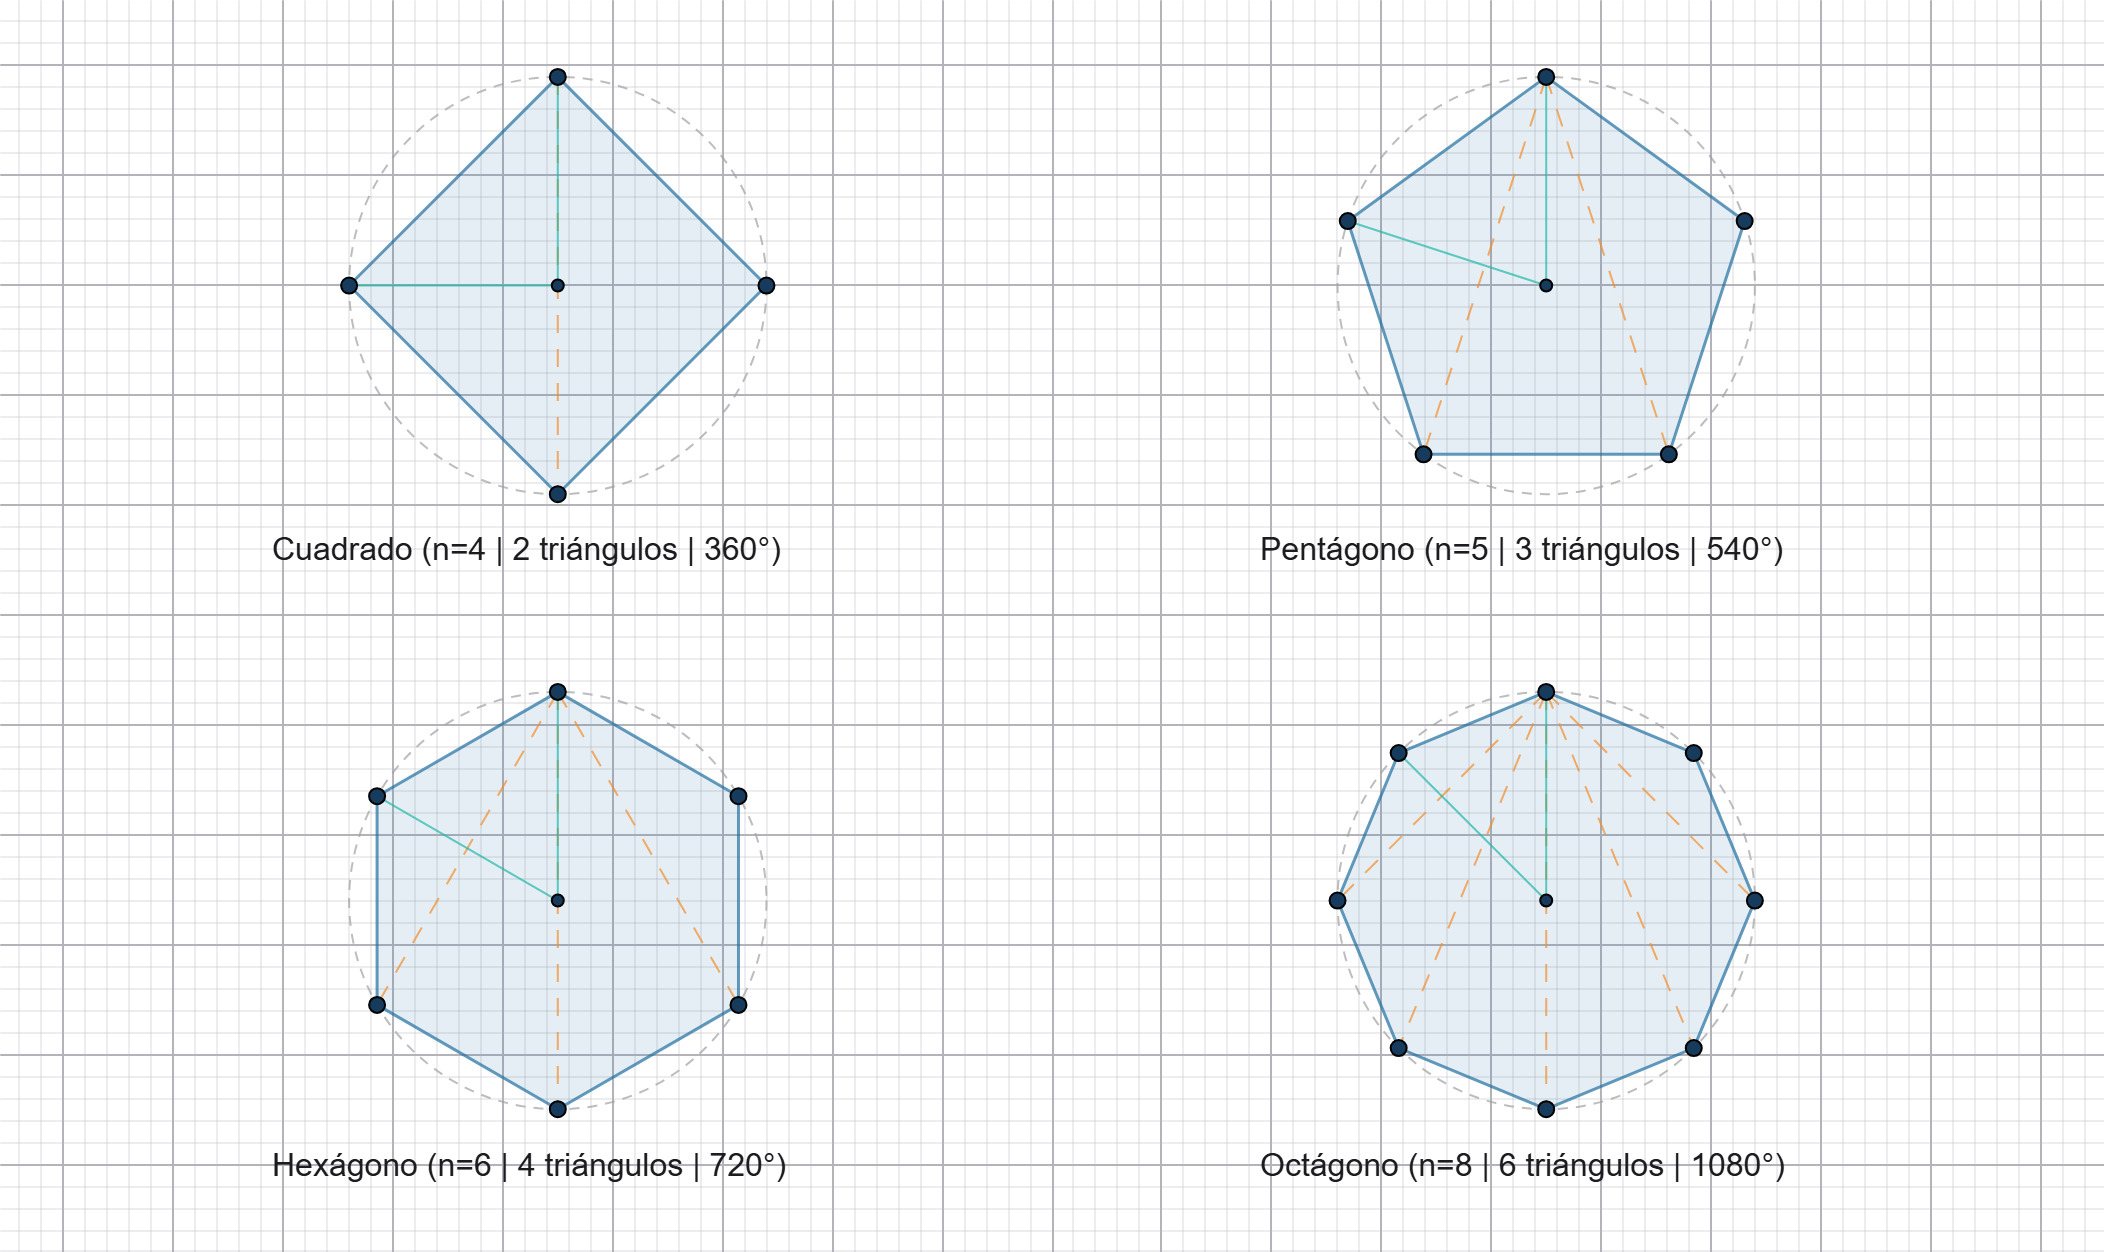
\includegraphics[width=0.84\linewidth]{img/geogebra/act3_poligonos_diagonales_angulos.png}
\caption{Construcción en GeoGebra: Triangulación por diagonales desde un vértice y ángulo central en polígonos regulares inscritos ($n=4,5,6,8$).}
\end{figure}

Como se analiza en la diapositiva 30, aunque al aumentar $n$ el contorno poligonal se aproxima asintóticamente a la circunferencia circunscrita, un polígono nunca se transforma literalmente en circunferencia: conserva siempre segmentos rectos, vértices y ángulos interiores discretos, mientras que la circunferencia es una curva continua sin lados rectos ni vértices.

\section{Exploración en GeoGebra: Ángulo central y ángulo inscrito}
Siguiendo el procedimiento de la diapositiva 32 y el Guión 3, se construyó una circunferencia con centro $O=(0,0)$, los puntos $A$ y $B$ en el arco superior, el ángulo central $\angle AOB$ y el punto $C$ en el arco inferior formando el ángulo inscrito $\angle ACB$. Se exploraron tres configuraciones dinámicas:

\begin{figure}[htbp]
\centering
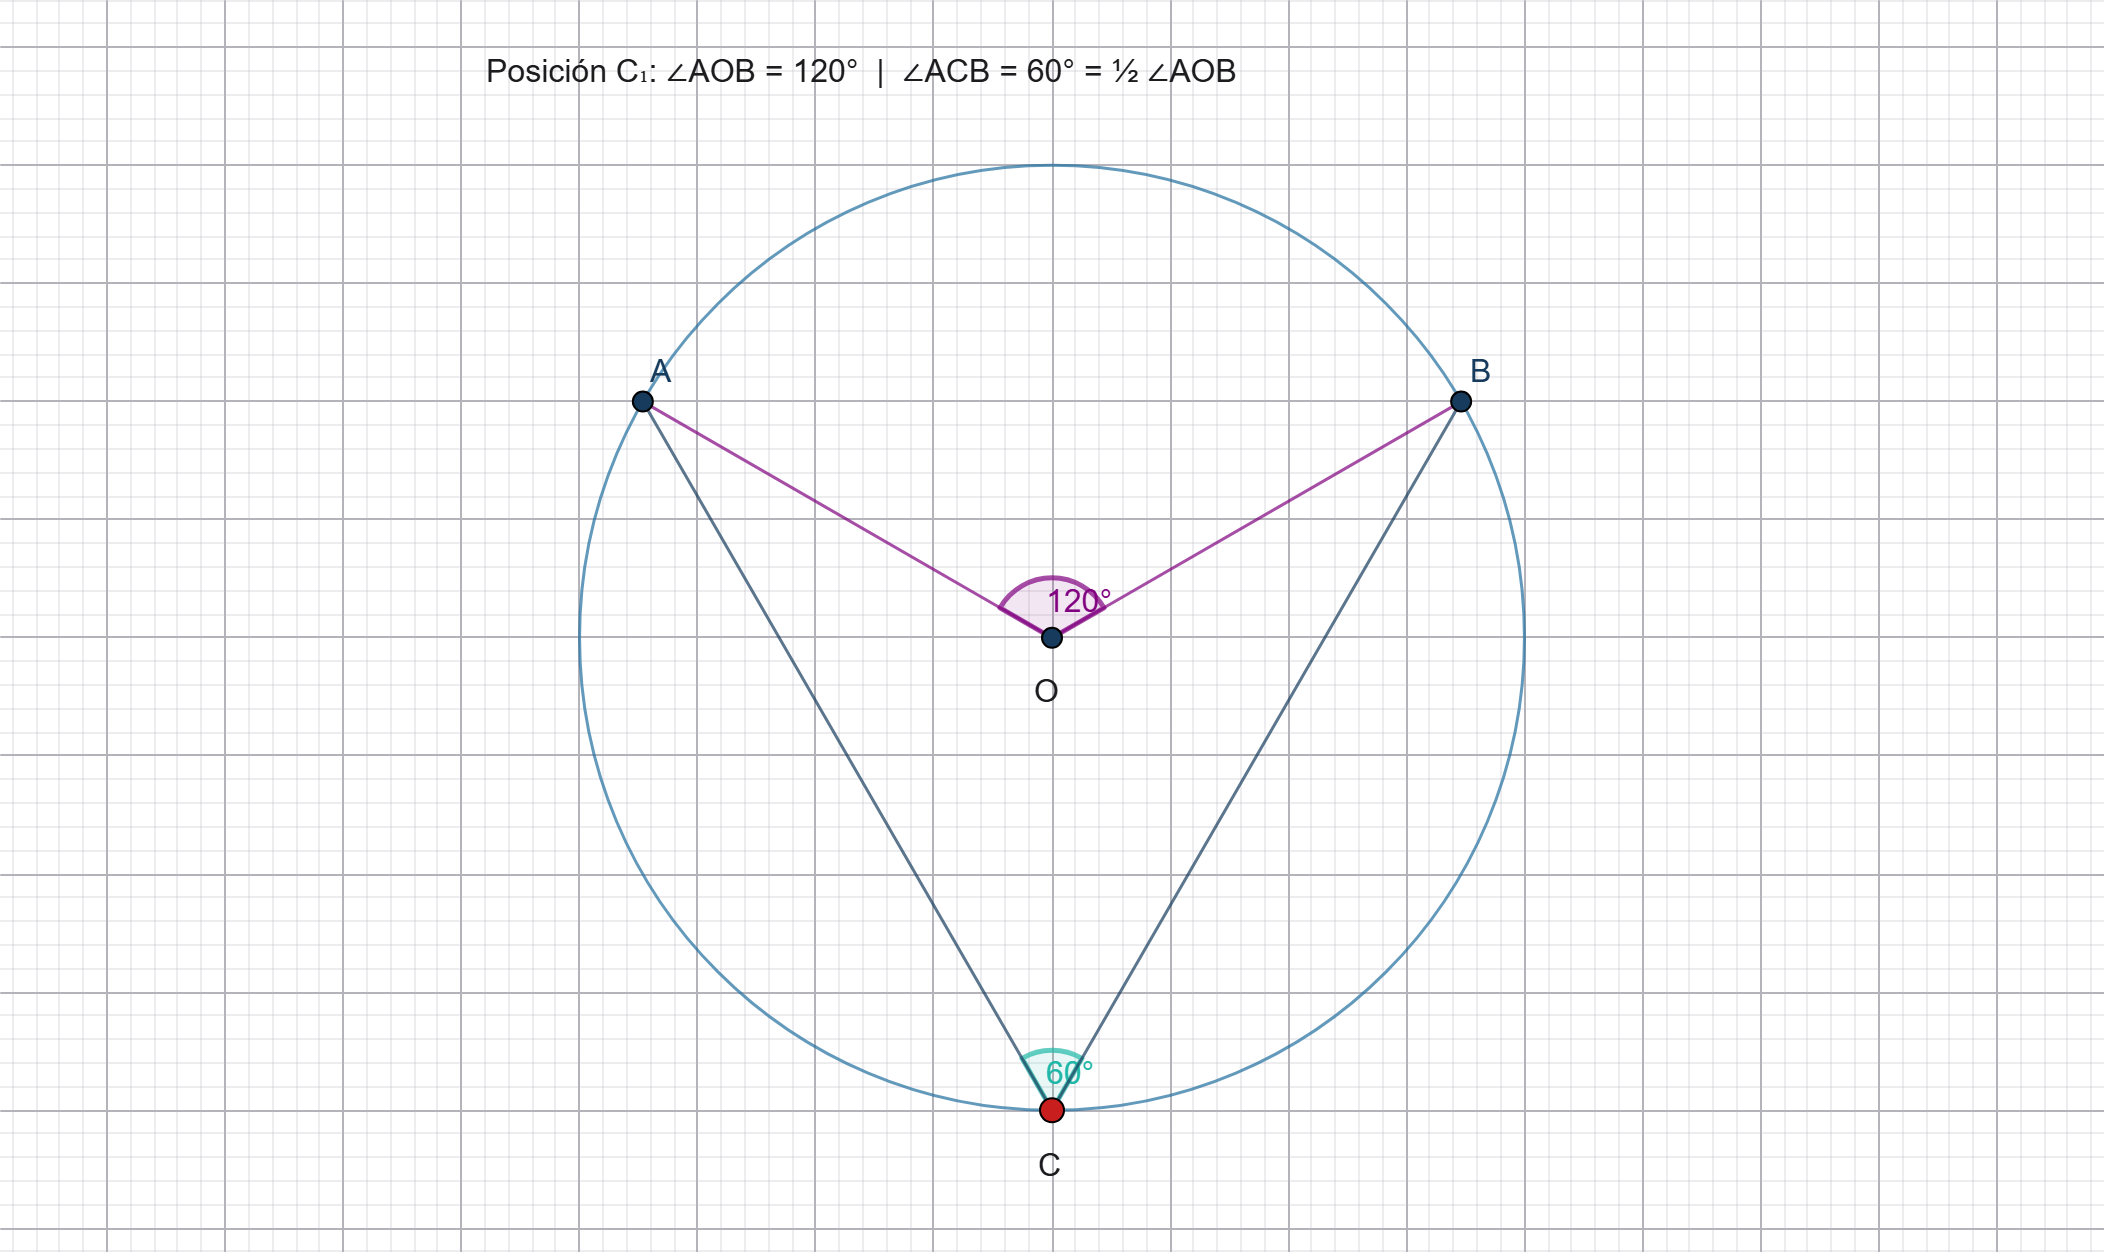
\includegraphics[width=0.32\linewidth]{img/geogebra/act3_angulo_central_inscrito_1.png}\hfill
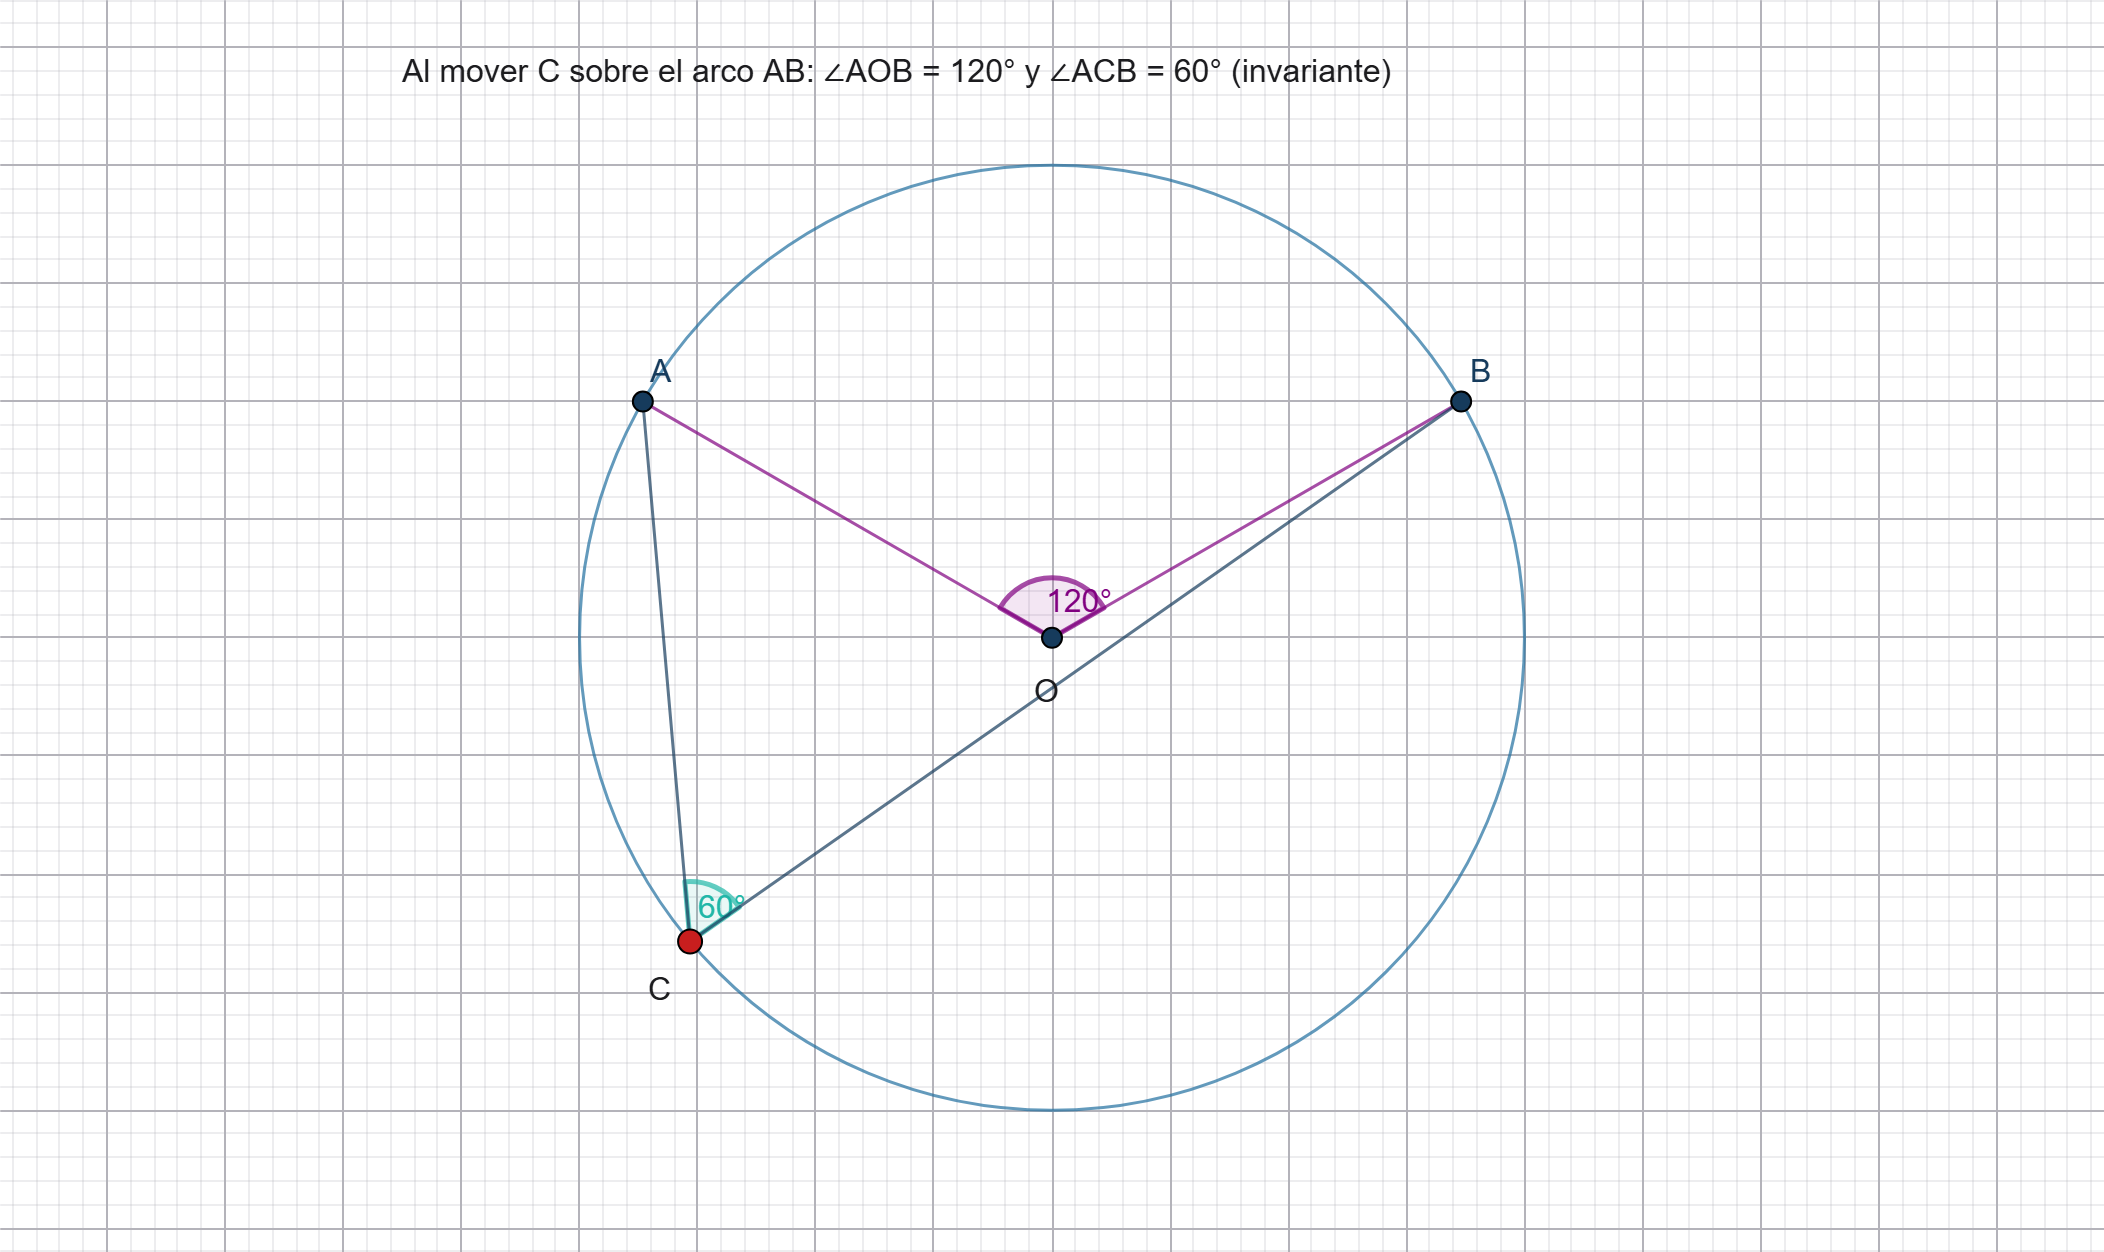
\includegraphics[width=0.32\linewidth]{img/geogebra/act3_angulo_central_inscrito_2.png}\hfill
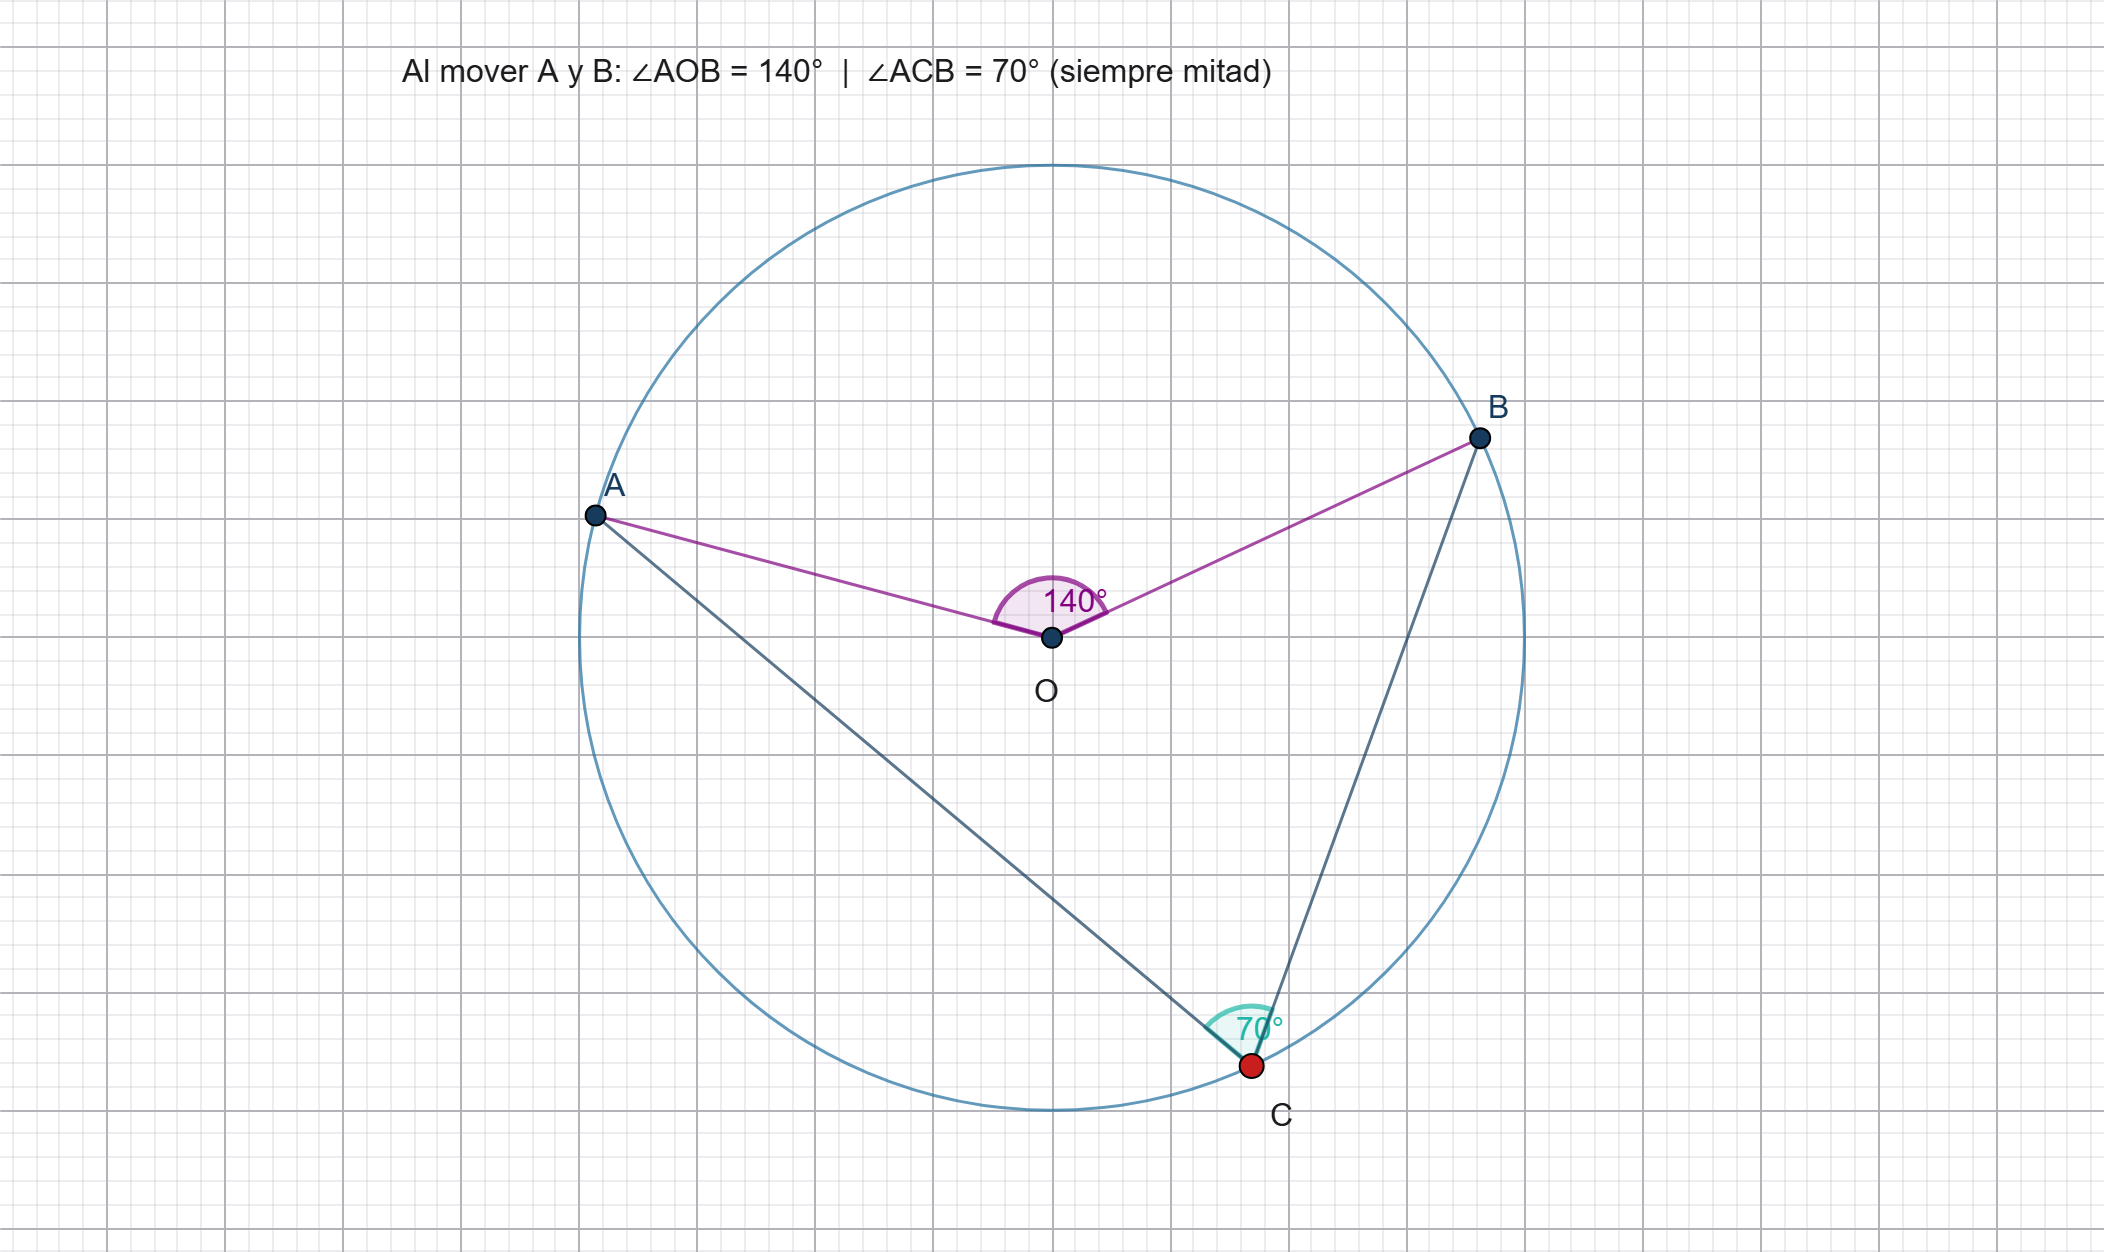
\includegraphics[width=0.32\linewidth]{img/geogebra/act3_angulo_central_inscrito_3.png}
\caption{Exploración dinámica en GeoGebra: (1) Posición inicial $C_1$ ($\angle AOB=120^\circ, \angle ACB=60^\circ$); (2) Desplazamiento de $C$ en el mismo arco manteniendo $\angle ACB=60^\circ$; (3) Cambio de arco $\overline{AB}$ ($\angle AOB=140^\circ, \angle ACB=70^\circ$).}
\end{figure}

\subsection{Respuestas a las preguntas de descubrimiento (Guión 3)}
\begin{enumerate}
  \item[\textbf{a.}] \textbf{¿Qué sucedió con la medida del ángulo inscrito al mover el punto $C$ sobre el mismo arco?} La medida del ángulo inscrito $\angle ACB$ \textbf{permaneció invariante} ($60^\circ$ en todas las posiciones sobre el arco inferior opuesto a $\widehat{AB}$).
  \item[\textbf{b.}] \textbf{¿Qué ocurrió con las medidas de ambos ángulos al cambiar la posición de $A$ o $B$?} Al variar el arco $\widehat{AB}$, la medida del ángulo central $\angle AOB$ cambió (por ejemplo de $120^\circ$ a $140^\circ$) y el ángulo inscrito $\angle ACB$ cambió simultáneamente en la misma proporción (de $60^\circ$ a $70^\circ$).
  \item[\textbf{c.}] \textbf{Relación numérica encontrada:} El ángulo inscrito que subtiende un arco mide exactamente \textbf{la mitad} del ángulo central correspondiente al mismo arco:
  \[
    \angle ACB = \frac{1}{2}\,\angle AOB.
  \]
  \textbf{Justificación matemática (demostración):} Trazando el diámetro auxiliar que pasa por $C$ y $O$ (cortando a la circunferencia en $D$), los triángulos $\triangle OAC$ y $\triangle OBC$ son isósceles porque $OA = OC = OB = r$. Si $\angle OCA = \alpha$, entonces $\angle OAC = \alpha$ y el ángulo exterior $\angle AOD = 2\alpha$. Análogamente, si $\angle OCB = \beta$, entonces $\angle OBC = \beta$ y $\angle BOD = 2\beta$. Sumando (o restando según la posición de $O$ respecto a los lados del ángulo inscrito), $\angle AOB = 2(\alpha + \beta) = 2\angle ACB$.
\end{enumerate}

\section{Reflexión pedagógica}
\begin{itemize}
  \item \textbf{Habilidades matemáticas desarrolladas:} Al construir polígonos, triangularlos e investigar ángulos en la circunferencia, el estudiante pone en juego la \textbf{visualización espacial}, la \textbf{medición}, la \textbf{inducción y generalización} de patrones numéricos ($(n-2)\cdot 180^\circ$ y $360^\circ/n$), la \textbf{comunicación} simbólica y la \textbf{deducción} mediante pruebas de invariancia.
  \item \textbf{Ventajas y limitaciones de GeoGebra en el aula:} Entre sus ventajas destacan la retroalimentación inmediata al arrastrar vértices, la posibilidad de verificar docenas de casos en segundos para distinguir propiedades invariantes de rasgos accidentales y la limpieza gráfica. Entre sus limitaciones figuran el riesgo de que el estudiante acepte la medición empírica como si sustituyera a la demostración deductiva, la brecha de equipamiento o conectividad en aulas públicas y la necesidad de mediar con preguntas para evitar el ensayo-error irreflexivo.
\end{itemize}

\needspace{5\baselineskip}\section*{Referencias}
{\setstretch{1.15}\setlength{\parskip}{6pt}
\par\hangindent=1.27cm\hangafter=1 Instituto de Investigación, Innovación y Estudios de Posgrado para la Educación del Estado de Nuevo León. (2026). \textit{Sesión 10: Universo 3-60. Presentación interactiva, Guión 3 y rúbrica de evaluación}. EVA Posgrados IIIEPE.
\par\hangindent=1.27cm\hangafter=1 Secretaría de Educación Pública. (2024). \textit{Programa de estudio para la educación secundaria: Programa sintético de la Fase 6}. SEP.
}

\end{document}
